\documentclass[11pt,a4paper]{article}

\usepackage[margin=1in]{geometry}
\usepackage[T1]{fontenc}
\usepackage[utf8]{inputenc}
\usepackage{lmodern}
\usepackage{amsmath,amssymb,amsthm}
\usepackage{booktabs}
\usepackage{graphicx}
\usepackage{microtype}
\usepackage{enumitem}
\usepackage{natbib}
\usepackage[hidelinks]{hyperref}
\usepackage{xurl}

\hypersetup{
  pdftitle={When Averaged Field Regularity Fails to Rank Few-Step Generative Paths},
  pdfauthor={Clément Callaert},
  pdfsubject={Commuting Gaussian probability-flow ODEs and averaged Jacobian regularity},
  pdfkeywords={flow matching, probability-flow ODE, few-step sampling, Wasserstein, Runge-Kutta}
}

\newcommand{\arxivReleaseTag}{arxiv-v1}
\newcommand{\arxivReleaseURL}{https://github.com/clement-callaert/fewstep-field-regularity/releases/tag/arxiv-v1}
\newcommand{\mpmathVersion}{1.3.0}
\newcommand{\nConfigs}{72}
\newcommand{\nBlocks}{36}
\newcommand{\nGeometries}{4}
\newcommand{\nSolverBudgets}{9}
\newcommand{\nInversions}{14}
\newcommand{\nWorkshopBlocks}{18}
\newcommand{\nWorkshopInversions}{11}
\newcommand{\nRobustLowRank}{66}
\newcommand{\scalarRlin}{0.9634954084936207}
\newcommand{\scalarRvp}{0.6168502750680849}
\newcommand{\scalarRlinClosed}{5\pi/8-1}
\newcommand{\scalarRvpClosed}{\pi^2/16}
\newcommand{\scalarRlinApprox}{0.9634954084936207}
\newcommand{\scalarRvpApprox}{0.6168502750680849}
\newcommand{\scalarRlinFrac}{6797469/3559400}
\newcommand{\scalarRlinFactor}{6797469/3559400}
\newcommand{\scalarWlin}{0.0902767320334888}
\newcommand{\scalarWvpLower}{0.1303736583}
\newcommand{\scalarWvpUpper}{0.1303736584}
\newcommand{\scalarRvpLo}{1.8696263416613175}
\newcommand{\scalarRvpHi}{1.8696263416613176}
\newcommand{\vpHeunBoundNum}{192113353671412470139303}
\newcommand{\vpHeunBoundDen}{102753427879939708813312}
\newcommand{\vpHeunIntLeft}{19211335367141247013930300}
\newcommand{\vpHeunIntRight}{19214891013548725548089344}
\newcommand{\strongRlin}{2.9441044083}
\newcommand{\strongRvp}{4.7305438136}
\newcommand{\strongRlinHat}{2.9476523251}
\newcommand{\strongRvpHat}{4.7295206355}
\newcommand{\strongWlin}{0.8108540111}
\newcommand{\strongWvp}{0.4564779075}
\newcommand{\strongMargin}{0.3543761036}
\newcommand{\smallMargin}{1.1188920612\times 10^{-5}}
\newcommand{\maxPrecDelta}{9.7050430488\times 10^{-10}}
\newcommand{\precRatio}{11528}
\newcommand{\lrTwoLmin}{0.2914701258115777}
\newcommand{\lrTwoLmax}{2.9677106074567434}
\newcommand{\nInversionCells}{5}
\newcommand{\nGeometrySolverCells}{12}
\newcommand{\nAllNFEInvertCells}{4}
\newcommand{\nDistinctRComparisons}{3}
\newcommand{\nLogcovWins}{36}
\newcommand{\RlinAniso}{0.972296}
\newcommand{\RvpAniso}{0.192270}


\newtheorem{proposition}{Proposition}
\newtheorem{definition}{Definition}
\newtheorem{assumption}{Assumption}
\theoremstyle{remark}
\newtheorem{remark}{Remark}

\newcommand{\wtwo}{W_2}
\newcommand{\RR}{\mathbb{R}}
\newcommand{\cR}{\mathcal{R}}
\newcommand{\EE}{\mathbb{E}}

\title{When Averaged Field Regularity Fails to Rank\\
Few-Step Generative Paths}
\author{%
  Clément Callaert\\
  CentraleSupélec and Université Paris-Saclay\\
  \texttt{callaert.clement@gmail.com}
}
\date{}

\begin{document}
\maketitle

\begin{abstract}
Choosing a probability path for few-step generative sampling is often guided by
an averaged regularity scalar of the velocity field: a path with smaller
averaged squared Jacobian norm is expected to discretize better at a fixed
budget of function evaluations (NFE). This paper studies that ranking question
in commuting Gaussian probability-flow ODEs, where endpoint laws and Gaussian
2-Wasserstein ($\wtwo$) errors are available in closed form, the regularity
integrand is analytically known, and sampling, training, and estimation noise
are absent. On a registered grid of \nConfigs{} equal-NFE configurations
(\nBlocks{} two-path comparisons) the averaged-regularity ordering of linear
versus variance-preserving paths does not determine the fixed-NFE $\wtwo$
ordering: \nInversions{} of \nBlocks{} blocks invert. The same phenomenon
appears in a separately specified non-centered commuting family
(\nWorkshopInversions{} of \nWorkshopBlocks{} blocks). All reported $\wtwo$
values and inversion orderings survive an 80-digit reference calculation.
An exact modal decomposition writes endpoint factor error as a transported sum
of signed, solver-stage-dependent local defects, information that an unsigned
time average of Jacobian norms cannot retain. An explicit scalar construction
proves the corresponding non-implication for fixed-grid left-endpoint Euler,
for every $L>0$ and every integer grid size $N\ge 1$. The construction is
grid-aware and is not offered as the mechanism of the Gaussian inversions.
The study is a controlled limitation: it does not refute regularity-guided
schedule design, and no learned model is evaluated. The counts
\nInversions{} of \nBlocks{} and \nWorkshopInversions{} of
\nWorkshopBlocks{} are descriptive benchmark frequencies, not estimates of a
population probability.
\end{abstract}

\section{Introduction}
\label{sec:intro}

Few-step sampling of a continuous-time generative model commits to a
probability path, a numerical solver, and a small NFE budget before any
endpoint error is observed. Classical one-step error bounds involve Lipschitz
and stability constants of the vector field~\citep{hairer1993solving}. In the
stochastic interpolant framework, \citet{lipschitzguided2025} propose
minimizing averaged squared drift Lipschitzness as a schedule criterion
(their Definition~3.2). Bounding an error, however, is weaker than determining
which of two paths errs less at an equal small budget.

This paper isolates that ranking question where it can be answered without
estimators. The systems are commuting Gaussian interpolants. The marginal
velocity is affine. A fixed-step Runge--Kutta method induces an affine
endpoint map, reconstructed from $d+1$ deterministic probes. Endpoint error is
the closed-form Gaussian $\wtwo$~\citep{gelbrich1990formula,peyre2019computational}.
The regularity scalar is a trapezoidal quadrature of an analytically known
spectral-norm integrand. Two paths are compared: the linear interpolant and
the trigonometric variance-preserving (VP) interpolant.

\textbf{Contributions.}
\begin{itemize}[leftmargin=1.4em]
  \item A controlled closed-form $\wtwo$ benchmark on commuting Gaussian
  flows: \nInversions{} inversions among \nBlocks{} equal-NFE comparisons in
  a registered grid of \nConfigs{} configurations, all 80-digit-verified, and
  a separately specified non-centered commuting family with
  \nWorkshopInversions{} inversions among \nWorkshopBlocks{} comparisons.
  \item An exact eigenmode analysis: the endpoint factor error is a
  transported sum of signed, solver-stage-dependent local defects.
  \item An explicit grid-aware smooth scalar construction proving that, for
  every $L>0$ and every integer $N\ge 1$, strictly larger averaged squared
  Jacobian is compatible with zero fixed-grid Euler endpoint error.
\end{itemize}

Solver dependence of good schedules is already documented in diffusion
practice~\citep{sabour2024align,karras2022edm}. The contribution here is the
exact, controlled non-implication and its modal accounting: what the tested
averaged-regularity scalar certifies, and what it discards, about
fixed-budget \emph{rankings} in these systems. Contemporaneous analyses of
strain versus vorticity and of material-derivative regularization
\citep{tao2026strain,khan2026isofm} address related numerical structure.
They do not study the linear-versus-VP ranking by averaged spectral Jacobian
on independent-coupling interpolants.

\begin{figure}[t]
  \centering
  
\includegraphics[width=\linewidth]{figures/fig1_conceptual.pdf}
  \caption{Conceptual schematic, not experimental data.
  (a)~Averaging collapses two time-dependent fields to two scalars, while a
  solver samples only stage locations (markers).
  (b)~Local defects are signed: same-sign defects accumulate, alternating
  defects cancel.
  (c)~After transport to the endpoint, the error ranking can oppose the
  averaged ranking.
  The panel illustrates the accounting of Section~\ref{sec:mechanism}, not
  the measured mechanism of any specific Gaussian inversion.}
  \label{fig:concept}
\end{figure}

\section{Background and problem formulation}
\label{sec:background}

\paragraph{Definition (interpolant).}
Let $X_0\sim N(\mu_0,\Sigma_0)$ and $X_1\sim N(\mu_1,\Sigma_1)$ be independent
in $\RR^d$, with $\Sigma_0,\Sigma_1$ symmetric positive definite. Let
$\alpha,\sigma:[0,1]\to\RR$ be $C^3$ scalar schedules. The interpolant is
\begin{equation}
  X_t=\alpha(t)X_0+\sigma(t)X_1,
  \label{eq:interpolant}
\end{equation}
as in stochastic interpolants and flow matching~\citep{albergo2025stochastic,lipman2023flow,liu2023rectified,tong2024conditional}.
The two schedules used as \emph{paths} in the benchmark are the linear path
$(\alpha,\sigma)=(1-t,\,t)$ and the trigonometric VP path
$(\cos(\pi t/2),\,\sin(\pi t/2))$, the interpolant analogue of VP diffusion
schedules~\citep{song2021score}.

\paragraph{Problem.}
Fix a solver from $\{\mathrm{Euler},\mathrm{Heun},\mathrm{RK4}\}$, an NFE
budget $B$ divisible by the solver's stage count, and two paths $b$ and $b'$.
Let $\cR$ be the averaged regularity scalar of Section~\ref{sec:regularity}
and let $E$ be the Gaussian $\wtwo$ endpoint error of
Section~\ref{sec:w2}. Does $\cR[b]<\cR[b']$ imply $E[b]<E[b']$?

The paper answers this in the negative for the tested commuting Gaussian
systems, as a logical and empirical non-implication, not as a claim about
learned neural fields.

\section{Gaussian probability paths and marginal velocity fields}
\label{sec:gaussian}

\paragraph{Assumption (independent Gaussian endpoints and positive definite
marginals).}
The endpoints are independent Gaussians as above, and
$Q(t):=\mathrm{Cov}(X_t)=\alpha(t)^2\Sigma_0+\sigma(t)^2\Sigma_1$ is
positive definite for every $t\in[0,1]$.

Under this assumption the marginal law of $X_t$ is Gaussian with mean
$m_t=\alpha\mu_0+\sigma\mu_1$. Differentiating the interpolant and taking the
Gaussian conditional expectation yields the affine marginal velocity
\begin{equation}
  b(t,x)=A(t)\,x+c(t),\qquad
  A(t)=C_t\,Q(t)^{-1},\qquad
  c(t)=\dot m_t-A(t)\,m_t,
  \label{eq:affine}
\end{equation}
with $C_t=\dot\alpha\alpha\,\Sigma_0+\dot\sigma\sigma\,\Sigma_1$.
This is the standard Gaussian conditional formula, written in the notation of
\citet[Example~3.3]{lipschitzguided2025} and extended to non-centered
non-isotropic endpoints. Invertibility of $Q(t)$ is required at every solver
stage.

\paragraph{Centered specialization.}
If $\mu_0=\mu_1=0$ and $\Sigma_0=I$, then $c\equiv 0$ and
$A(t)=\tfrac12 Q'(t)Q(t)^{-1}$.

\paragraph{Assumption (commuting covariance flow).}
Throughout the benchmark, $\Sigma_0=I$ and $\Sigma_1$ is simultaneously
diagonalized with $I$. Then $Q(t)$, $Q'(t)$, and $A(t)$ commute. In the
eigenbasis of $\Sigma_1$, mode $i$ with eigenvalue $\lambda_i>0$ obeys
$x_i'=a_i(t)x_i+c_i(t)$ with
$q_i(t)=\alpha(t)^2+\lambda_i\sigma(t)^2$ and
$a_i(t)=q_i'(t)/(2q_i(t))$ when $\Sigma_0=I$.
The exact one-step factor on $[t_n,t_{n+1}]$ is
$\sqrt{q_i(t_{n+1})/q_i(t_n)}$. For centered modes,
$q_i(0)=1$ and $q_i(1)=\lambda_i$, so the exact endpoint factor is
$\sqrt{\lambda_i}$.

This commuting hypothesis is essential. Noncommuting covariance flows are
outside the theorems and the tables.

\section{Averaged field regularity and fixed-budget error}
\label{sec:regularity}

\paragraph{Definition (averaged regularity scalar).}
Following \citet[Definition~3.2]{lipschitzguided2025},
\begin{equation}
  \cR[b]=\int_0^1 \bigl\|A(t)\bigr\|_2^2\,dt
  \label{eq:R}
\end{equation}
for the affine field~\eqref{eq:affine}, where $\|\cdot\|_2$ is the matrix
spectral norm. For state-independent $A(t)$ this coincides with the path
expectation in their Eq.~(3.4). By definition $\cR$ ignores $c(t)$.

\paragraph{Numerical evaluation (not an exact integral).}
In every reported number, $\cR$ is a trapezoidal quadrature of the
analytically known integrand on $24$ uniform nodes in $[0,1]$. The
implementation records this quantity as non-exact. Rankings in the
registered grid are nevertheless strict: no comparison block has a tied
$\cR$ value.

\paragraph{Definition (equal-NFE accounting).}
Euler uses $1$ field evaluation per step, Heun $2$, and classical RK4 $4$.
A requested budget $B$ is admitted only if $B$ is divisible by the stage
count $s$. The step count is $S=B/s$. The time grid is the uniform partition
of $[0,1]$ with $S$ steps, including both endpoints. Jacobian evaluations
used for metrics are not counted as NFE. Equal NFE is not equal step count:
at $B=8$, Euler takes $8$ steps, Heun $4$, and RK4 $2$.

\paragraph{Definition (endpoint error).}
\label{sec:w2}
A solver applied to~\eqref{eq:affine} produces an affine endpoint map
$x\mapsto Rx+d$, recovered from the images of $0$ and the canonical basis.
Source moments are pushed through this map. Error is the Gaussian
$\wtwo$~\citep{gelbrich1990formula,peyre2019computational},
\begin{equation}
  \wtwo^2=\|m-\mu_1\|_2^2
  +\mathrm{tr}\bigl(C+\Sigma_1-2(\Sigma_1^{1/2}C\Sigma_1^{1/2})^{1/2}\bigr),
\end{equation}
with PSD square roots. In the centered commuting case, if $r_i$ is the
numerical endpoint factor of mode $i$,
\begin{equation}
  \wtwo^2=\sum_i\bigl(|r_i|-\sqrt{\lambda_i}\bigr)^2.
  \label{eq:modalw2}
\end{equation}
The absolute value appears because the PSD square root of $r_i^2$ is $|r_i|$.
This is endpoint \emph{distribution} error, not trajectory error.

Reported float64 values are compared with an 80-digit \texttt{mpmath}
propagation of the same modal maps. The comparison is a precision audit, not
a second experiment.

\section{Exact solver-stage and modal error analysis}
\label{sec:mechanism}

Let $e_{i,n}=\sqrt{q_i(t_{n+1})/q_i(t_n)}$ be the exact factor of mode $i$
and let $r_{i,n}$ be the numerical one-step factor (Appendix~\ref{app:solvers}).
For nonzero factors the algebraic identity
\begin{equation}
  \prod_{n=0}^{S-1} r_{i,n}-\prod_{n=0}^{S-1} e_{i,n}
  =\sum_{n=0}^{S-1}(r_{i,n}-e_{i,n})
  \Bigl(\prod_{j<n}r_{i,j}\Bigr)
  \Bigl(\prod_{j>n}e_{i,j}\Bigr)
  \label{eq:telescope}
\end{equation}
holds with no smallness or positivity assumption. Prefixes are numerical;
suffixes are exact. This is the transported signed-defect decomposition.

For smooth $a$, the leading exact-minus-method coefficients are
$\tfrac12(a'+a^2)h^2$ for Euler and
$\bigl(-\tfrac1{12}a''+\tfrac16 a^3\bigr)h^3$ for the implemented Heun
method (Appendix~\ref{app:lte}). They involve different derivatives, signs,
and stage locations. Classical RK4 cancels all lower-order terms; no closed
RK4 coefficient is asserted.

Identity~\eqref{eq:telescope} identifies what $\cR$ discards: which times
the stages sample, the derivatives of $A$, the signs of local defects, their
cancellation, and their transport to the endpoint. An unsigned average of
$\|A\|_2^2$ therefore need not determine the fixed-NFE ordering. This is an
accounting statement. It is not, by itself, a proof that any particular
Gaussian pair inverts.

\section{Controlled benchmark}
\label{sec:benchmark}

\paragraph{Registered grid.}
Source $N(0,I)$. Targets: anisotropic Gaussians with condition number $4$,
and seeded low-rank Gaussians $FF^\top+0.05 I$ with rank $2$ and geometry
seed $271828$. Dimensions $d\in\{2,8\}$. Paths: linear and VP. Solvers:
Euler, Heun, RK4. NFE $\in\{8,16,32\}$ with equal-NFE accounting.
This is $\nConfigs{}$ float64 CPU configurations in $\nBlocks{}$ two-path
blocks. Mixture targets are excluded: dimension-$8$ mixture endpoint
estimators failed a post-result calibration diagnostic, and Phase~4
reproduction accepts Gaussian targets only.

\paragraph{Inversion.}
A block is an inversion when the strict $\cR$ ordering disagrees with the
strict $\wtwo$ ordering. There are no ties in this grid.

\paragraph{Chronology.}
Inversions were first identified in a registered broader gate benchmark,
then the Gaussian grid above was frozen and rerun from clean code. The
decomposition, local-error proxies, extra NFE budgets, and perturbations
are post-hoc relative to that gate. A non-centered family was specified in
writing before its result commit (Section~\ref{sec:empirical}).

\section{Main empirical results}
\label{sec:empirical}

All \nConfigs{} rows reproduce the registered precursor within absolute
tolerance $10^{-12}$. Independent grouping of the frozen
\texttt{results.json} yields \nInversions{} inversions among \nBlocks{}
blocks (Figure~\ref{fig:inversions}; full list in
Table~\ref{tab:allinv} of the appendix). These are descriptive counts on
the tested grid.

In the strongest inversion (low-rank, $d=8$, Euler, NFE $8$;
Table~\ref{tab:strongest}), $\cR$ prefers linear while $\wtwo$ prefers VP,
with margin $\strongMargin$. All \nConfigs{} float64 $\wtwo$ values agree
with the 80-digit reference to at most $\maxPrecDelta$. The smallest
inversion margin, $\smallMargin$ (low-rank, $d=2$, RK4, NFE $32$), is
$\precRatio$ times that global precision gap. Every inverted block keeps
the same $\wtwo$ ordering at 80 digits.

\begin{table}[t]
  \centering
  \caption{Strongest inversion in the registered grid: low-rank Gaussian,
  $d=8$, Euler, NFE $8$. Values are generated from the frozen artifact;
  $\cR$ is trapezoidal with $24$ nodes. Lower $\cR$ is the regularity
  preference; lower $\wtwo$ is the error preference. The table supports a
  ranking disagreement on this block. It does not support a universal
  preference for VP.}
  \label{tab:strongest}
  \begin{tabular}{lcc}
    \toprule
    path & $\cR[b]$ & Gaussian $\wtwo$ \\
    \midrule
    linear & $\mathbf{\strongRlin}$ & $\strongWlin$ \\
    variance-preserving & $\strongRvp$ & $\mathbf{\strongWvp}$ \\
    \bottomrule
  \end{tabular}
\end{table}

\begin{figure}[t]
  \centering
  
\includegraphics[width=\linewidth]{figures/fig2_inversions.pdf}
  \caption{Left and middle: strongest inversion in both quantities;
  hatching marks VP. Right: $\wtwo$ margins of all \nInversions{} inversion
  blocks on a logarithmic axis (which compresses, never exaggerates,
  magnitudes). Marker shape and color give the $\wtwo$-preferred path.
  Source: frozen Phase~4 reproduction, \nBlocks{} blocks.}
  \label{fig:inversions}
\end{figure}

\paragraph{Solver--path interaction (low-rank family only).}
On all $18$ low-rank primary blocks, VP has smaller $\wtwo$ under Euler and
linear has smaller $\wtwo$ under Heun and RK4, at both dimensions and every
primary budget (Figure~\ref{fig:interaction}). The pattern persists on a
post-hoc robustness grid with NFE $64$ and $128$ and with $\pm 10\%$ target
perturbations ($66$ of $66$ low-rank robustness blocks). Solver-dependent
schedule preference is known~\citep{sabour2024align}. Here the tested
averaged-regularity scalar does not capture the interaction. The split is
not claimed for the anisotropic family, whose primary inversions are
Heun-only.

\begin{figure}[t]
  \centering
  
\includegraphics[width=\linewidth]{figures/fig3_interaction.pdf}
  \caption{Signed low-rank $\wtwo$ margin at equal NFE. Positive values
  prefer VP; negative values prefer linear. The axis is symmetric-log
  (linear threshold $10^{-4}$) because margins span several orders of
  magnitude and change sign. The figure supports a solver-dependent
  preference on this family and these budgets. It does not establish a
  schedule rule outside the tested systems.}
  \label{fig:interaction}
\end{figure}

\paragraph{Non-centered supporting family.}
Before execution, one additional family was frozen: source
$N(\mu_0,I)$ with $\mu_{0,i}=0.75(-1)^i$; target $N(\mu_1,D)$ with
$\mu_{1,i}=1+0.25i$ and $D$ diagonal, geometric eigenvalues, condition
number $6$. Then $c(t)\ne 0$ in~\eqref{eq:affine}. The same paths, solvers,
and budgets give \nWorkshopBlocks{} blocks. A documented amendment between
the freeze and the result commit changed only the endpoint sanity check
(moment gap instead of a $\wtwo$ threshold that float64 identical Gaussians
cannot meet). The family itself was not changed.

\nWorkshopInversions{} of \nWorkshopBlocks{} blocks invert.
$\cR$, which ignores $c(t)$, prefers VP with margin $\workshopRmargin$;
$\wtwo$ prefers linear on the inverted blocks. All inverted blocks pass the
80-digit audit (maximum float64 deviation $\workshopPrecDelta$; smallest
inverted margin $\workshopSmallMargin$). The family remains Gaussian,
diagonal, and commuting. It is one supporting replication, not
out-of-distribution evidence.

\paragraph{Post-hoc local-error proxy.}
On the same \nBlocks{} centered blocks, $\cR$ agrees with the observed
$\wtwo$ preference in $22$ blocks. A solver-specific leading local-error
proxy agrees in $29$ blocks. That comparison is post-hoc and in-sample. It
is not a predictive claim. Exact transported defects account for endpoint
factor error by~\eqref{eq:telescope}.

\begin{figure}[t]
  \centering
  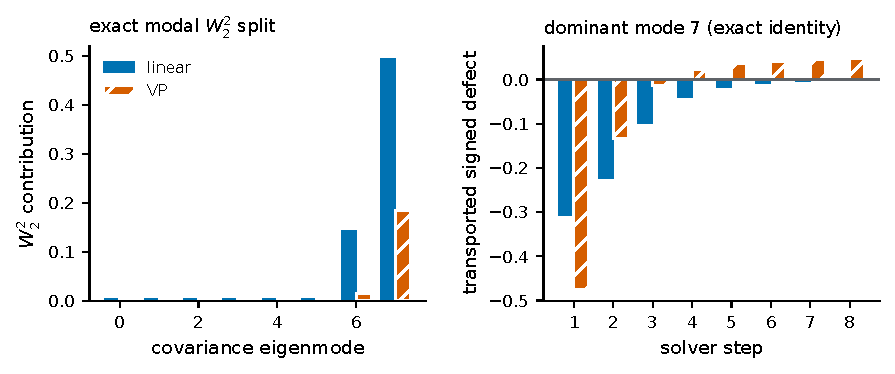
\includegraphics[width=\linewidth]{figures/fig_eigenmode.pdf}
  \caption{Exact modal $\wtwo^2$ contributions and transported signed local
  defects on the dominant mode for the strongest comparison. The
  decomposition is an identity on the recorded factors. Aggregate solver
  proxies are not shown as predictive.}
  \label{fig:eigenmode}
\end{figure}

\section{Fixed-grid Euler non-implication}
\label{sec:prop}

\begin{proposition}
\label{prop:euler}
Fix $L>0$ and an integer $N\ge 1$. Let $h=1/N$ and let forward Euler use the
left-endpoint grid $t_n=nh$ on $[0,1]$. Set
$\varepsilon_N=N(e^{L/N}-1)-L>0$ and define $f_k(t,x)=a_k(t)x$ with
$a_0(t)=L$ and $a_{1,N}(t)=L+\varepsilon_N\cos(2\pi Nt)$. For $x(0)=1$:
(i) both exact endpoints equal $e^{L}$;
(ii) $\int_0^1 a_{1,N}^2=L^2+\varepsilon_N^2/2>\int_0^1 a_0^2$;
(iii) Euler is exact for $a_{1,N}$;
(iv) Euler has strictly positive endpoint error for $a_0$.
Hence larger averaged squared Jacobian does not imply larger fixed-grid
Euler endpoint error.
\end{proposition}

\begin{proof}
(i) $\int_0^1\cos(2\pi Nt)\,dt=0$ for integer $N$, so both coefficients
integrate to $L$ and $x(1)=e^{L}$.
(ii) Orthogonality gives the displayed integrals, and $\varepsilon_N>0$
because $e^{z}>1+z$ for $z=L/N>0$.
(iii) $\cos(2\pi Nt_n)=1$ at every left node, so each Euler factor equals
$e^{L/N}$ and the product is $e^{L}$.
(iv) $\log(1+z)<z$ for $z>0$ yields $(1+L/N)^N<e^{L}$.
\end{proof}

The quantifiers matter. The field $a_{1,N}$ is chosen after the grid. Its
amplitude vanishes as $N\to\infty$. Shifted grids and multi-stage solvers
sample different phases. The construction shows non-implication for
fixed-grid left-endpoint Euler only. It is not the mechanism behind every
Gaussian inversion, and it is not presented as a new numerical-analysis
phenomenon. Edge cases, including $N=1$ and the exclusion of $L=0$, are
recorded in Appendix~\ref{app:p4p1}. An 80-digit check confirms that the
oscillatory Euler product equals $e^{L}$.

\section{Relation to existing schedule and solver design}
\label{sec:related}

Flow matching and stochastic interpolants supply the Gaussian path family
and its fields~\citep{lipman2023flow,albergo2025stochastic,liu2023rectified,tong2024conditional}.
Lipschitz-guided schedule design proposes the criterion tested
here~\citep{lipschitzguided2025}. Fast diffusion solvers exploit exactly
integrated linear parts and solver-specific
expansions~\citep{lu2022dpmsolver,lu2022dpmsolverpp,zhang2023deis}. EDM
separates schedule from discretization~\citep{karras2022edm}, and Align Your
Steps tunes schedules per solver, model, and dataset~\citep{sabour2024align}.
Runge--Kutta and backward error analysis supply the local-error
machinery~\citep{butcher1963coefficients,hairer1993solving,hairer2006geometric}.

\citet{tao2026strain} decompose Jacobian strain and vorticity in flow-matching
integration error and prove that McCann displacement interpolation has
vanishing material derivative, so Euler is exact on those Lagrangian
trajectories. The paths in the present benchmark are independent-coupling
interpolants, not McCann maps, so that exactness result does not apply to
the linear and VP fields used here. \citet{khan2026isofm} regularize the
material derivative of learned fields. Neither paper produces the commuting
inversion table or Proposition~\ref{prop:euler}.

A literature search on 2026-08-13 (arXiv and the sources listed in the
accompanying audit) did not locate an identical commuting Gaussian ranking
counterexample. Search absence is not a proof that none exists.

\section{Limitations and scope}
\label{sec:limits}

The systems are closed-form commuting affine Gaussian flows with two paths,
three fixed-step solvers, $d\in\{2,8\}$, small equal-NFE budgets, and one
non-centered commuting replication. No learned neural field is evaluated.
No image, video, or world-model quantity is reported. Mixture targets were
excluded after estimator calibration failure; they do not support any
conclusion here. Proposition~\ref{prop:euler} is grid-aware and Euler-only.
Exponential and exact-linear integrators solve affine scalar modes exactly,
so the numerical comparisons concern generic fixed-stage Runge--Kutta
discretization. Robustness NFE $64$ and $128$ and $\pm 10\%$ perturbations
are post-hoc. The leading local-error proxy is post-hoc and in-sample.

The result does not refute Lipschitz-guided schedules. In the tested
systems the averaged-regularity \emph{ordering} does not determine the
fixed-NFE $\wtwo$ ordering, because the tested scalar does not retain
solver-stage sampling, signs, cancellation, or transport.

\section{Conclusion}
\label{sec:conclusion}

On a registered commuting Gaussian grid, ordering two interpolants by
trapezoidal averaged squared Jacobian does not determine their equal-NFE
Gaussian $\wtwo$ ordering. The mismatch is visible in
\nInversions{} of \nBlocks{} blocks and in
\nWorkshopInversions{} of \nWorkshopBlocks{} blocks of a specified
non-centered family, and it is compatible with an exact transported-defect
identity and with a grid-aware Euler non-implication. The statement is as
narrow as the evidence.

\section{Reproducibility statement}
\label{sec:repro}

\begin{sloppypar}
Default analytical precision is float64. Figures and numerical macros in
this PDF are generated by \texttt{scripts/make\_arxiv\_figures.py} and
\texttt{scripts/make\_arxiv\_tables.py} from checksum-pinned JSON artifacts.
The primary artifact
\path{phase4_gaussian_reproduction_2026-07-24-v1:results}
has SHA-256 {\footnotesize\texttt{\primarySha}}.
Validate a run directory with
\path{python scripts/validate_artifacts.py outputs/<run_id>}.
Tests: \texttt{pytest}. Release-ready runs refuse a dirty worktree.
Code commit for this manuscript audit: {\footnotesize\texttt{\auditCommit}}.
Repository:
\url{https://github.com/clement-callaert/fewstep-field-regularity}.
\end{sloppypar}

\bibliographystyle{plainnat}
\bibliography{references}

\appendix
\section{Solver formulas and equal-NFE accounting}
\label{app:solvers}

On a step $[t,t+h]$ for $x'=a(t)x$, the implemented factors are
\begin{align}
  r_{\mathrm{Euler}}&=1+ha(t),\\
  r_{\mathrm{Heun}}&=1+\tfrac h2\bigl(a(t)+a(t+h)(1+ha(t))\bigr),
\end{align}
and classical RK4 with stages at $t$, $t+h/2$ (twice), and $t+h$. These match
the vector solvers applied to affine fields. Equal-NFE requires
$B\equiv 0\pmod s$ and sets $S=B/s$.

\section{Local truncation expansions}
\label{app:lte}

Assume $a$ is $C^3$. The exact factor admits the Taylor expansion
$1+ha+(h^2/2)(a'+a^2)+(h^3/6)(a''+3aa'+a^3)+O(h^4)$. Subtracting the Euler
factor leaves $\tfrac12(a'+a^2)h^2+O(h^3)$. Substituting the Taylor expansion
of $a(t+h)$ into the implemented Heun factor and subtracting from the exact
series leaves $\bigl(-a''/12+a^3/6\bigr)h^3+O(h^4)$. The $aa'$ terms cancel.
This expansion was confirmed with independent symbolic algebra on the
implemented expression. RK4 is compared numerically to the exact factor; no
memorized non-autonomous RK4 coefficient is used.

\section{Proof details for Proposition~\ref{prop:euler}}
\label{app:p4p1}

The body proof is complete for the stated quantifiers. Additional remarks:
$N=1$ holds, with $\varepsilon_1=e^{L}-1-L$ and a single Euler factor
$e^{L}$. The case $L=0$ is excluded because the metric ordering is not
strict. As $N\to\infty$ with $L$ fixed, $\varepsilon_N=L^2/(2N)+O(N^{-2})$,
so the oscillatory amplitude vanishes. Every Euler factor in the construction
is positive. An 80-digit evaluation of $(1+h(L+\varepsilon_N))^N$ equals
$e^{L}$ to working precision for representative pairs including $(L,N)=(1,8)$.
The construction does not apply to Heun, RK4, right-endpoint Euler, or a
fixed oscillatory ODE under grid refinement.

\section{Full inversion tables}
\label{app:tables}

Table~\ref{tab:allinv} lists every inverted block in the registered centered
grid. Table~\ref{tab:workshop} lists every comparison block in the
non-centered family. Both tables are generated from pinned artifacts.

\begin{table}[ht]
  \centering
  \caption{All \nInversions{} inversions among \nBlocks{} centered blocks.
  Margins are absolute Gaussian $\wtwo$ differences. Descriptive grid counts
  only.}
  \label{tab:allinv}
  \small
  \begin{tabular}{llcccrr}
\toprule
family & $d$ & solver & NFE & $R$ prefers & $W_2$ prefers & $W_2$ margin \\
\midrule
anisotropic & 2 & heun & 8 & VP & linear & $1.905310\times 10^{-3}$ \\
anisotropic & 2 & heun & 16 & VP & linear & $1.939806\times 10^{-3}$ \\
anisotropic & 2 & heun & 32 & VP & linear & $6.634439\times 10^{-4}$ \\
anisotropic & 8 & heun & 16 & VP & linear & $1.758942\times 10^{-3}$ \\
anisotropic & 8 & heun & 32 & VP & linear & $7.628173\times 10^{-4}$ \\
factor+noise & 2 & heun & 8 & VP & linear & $1.836251\times 10^{-2}$ \\
factor+noise & 2 & heun & 16 & VP & linear & $6.039925\times 10^{-3}$ \\
factor+noise & 2 & heun & 32 & VP & linear & $1.698035\times 10^{-3}$ \\
factor+noise & 2 & rk4 & 8 & VP & linear & $1.516722\times 10^{-3}$ \\
factor+noise & 2 & rk4 & 16 & VP & linear & $1.289981\times 10^{-4}$ \\
factor+noise & 2 & rk4 & 32 & VP & linear & $1.118892\times 10^{-5}$ \\
rank-2 factor+noise & 8 & euler & 8 & linear & VP & $3.543761\times 10^{-1}$ \\
rank-2 factor+noise & 8 & euler & 16 & linear & VP & $2.046946\times 10^{-1}$ \\
rank-2 factor+noise & 8 & euler & 32 & linear & VP & $1.096576\times 10^{-1}$ \\
\bottomrule
\end{tabular}

\end{table}

\begin{table}[ht]
  \centering
  \caption{Non-centered family: all \nWorkshopBlocks{} blocks.
  Positive $R_{\mathrm{lin}}-R_{\mathrm{VP}}$ means $\cR$ prefers VP.
  Negative $W_2$ difference means $\wtwo$ prefers linear.}
  \label{tab:workshop}
  \small
  \begin{tabular}{cccccl}
\toprule
$d$ & solver & NFE & inversion & $W_2$ prefers & $W_2^2$ driver \\
\midrule
2 & euler & 8 & no & VP & covariance \\
2 & euler & 16 & no & VP & covariance \\
2 & euler & 32 & no & VP & covariance \\
2 & heun & 8 & yes & linear & mean \\
2 & heun & 16 & yes & linear & mean \\
2 & heun & 32 & yes & linear & covariance \\
2 & rk4 & 8 & no & VP & covariance \\
2 & rk4 & 16 & no & VP & covariance \\
2 & rk4 & 32 & yes & linear & covariance \\
8 & euler & 8 & yes & linear & mean \\
8 & euler & 16 & yes & linear & mean \\
8 & euler & 32 & yes & linear & mean \\
8 & heun & 8 & yes & linear & mean \\
8 & heun & 16 & yes & linear & mean \\
8 & heun & 32 & yes & linear & mean \\
8 & rk4 & 8 & no & VP & covariance \\
8 & rk4 & 16 & no & VP & covariance \\
8 & rk4 & 32 & yes & linear & mean \\
\bottomrule
\end{tabular}

\end{table}

\section{Precision-audit method}
\label{app:precision}

Each modal factor is recomputed in \texttt{mpmath} at $80$ decimal digits
with the same stage formulas. Gaussian $\wtwo$ is formed from those factors.
The recorded maximum absolute float64-versus-reference difference on the
centered grid is $\maxPrecDelta$, below the pre-set tolerance $2\times 10^{-9}$.
A distinct residual, $\reconResidual$, measures eigenmode
reconstruction of float64 $\wtwo$ and is not the 80-digit gap.

\section{Excluded mixture experiments}
\label{app:mixtures}

Phase~2 and Phase~3 contain Gaussian-mixture runners and sliced-Wasserstein
estimators. Dimension-$8$ mixture blocks failed a post-result calibration
diagnostic and were excluded from decision evidence. Dimension-$2$ two-mode
blocks were used only in a gate condition and are not part of the Phase~4
conclusion. Phase~4 reproduction refuses non-Gaussian targets.

\section{Artifact map and reproduction commands}
\label{app:artifacts}

\begin{center}
\small
\begin{tabular}{ll}
\toprule
alias & artifact \\
\midrule
A1 & \texttt{phase4\_gaussian\_reproduction\_2026-07-24-v1:results} \\
A2 & \texttt{phase4\_precision\_2026-07-24-v1:table} \\
A3 & \texttt{phase4\_diagnostics\_2026-07-24-v1:table} \\
A4 & \texttt{phase4\_robustness\_2026-07-24-v1:table} \\
A5--A7 & external-validation results, inversions, precision \\
\bottomrule
\end{tabular}
\end{center}

\noindent
Install with Python $3.11+$ and then:
\begin{verbatim}
python -m pip install -e ".[dev]"
pytest
python scripts/validate_artifacts.py \
  outputs/phase4_gaussian_reproduction_2026-07-24-v1
python scripts/make_arxiv_tables.py
python scripts/make_arxiv_figures.py
\end{verbatim}
Release-ready experiment reruns require a clean worktree and
\texttt{overwrite: false}.

\end{document}
